%You can delete all the comments after you have finished your document
%this sets up the defaults for the documents, 12pt font and A4 size. The article type sets this up as such as opposed to letter or memo.

%for the finer points LaTeX see https://en.wikibooks.org/wiki/LaTeX or http://tex.stackexchange.com/

\documentclass[12pt,a4paper]{article}
\usepackage{titlesec} %these are how we import packages, one helps set up footers and title layout
\usepackage{fancyhdr}

% !TEX TS-program = pdflatex
% !TEX encoding = UTF-8 Unicode
\usepackage[utf8]{inputenc} % set input encoding (not needed with XeLaTeX)

\usepackage{graphicx} % support the \includegraphics command and options
\graphicspath{ {./images/} }
% \usepackage[parfill]{parskip} % Activate to begin paragraphs with an empty line rather than an indent

%%% PACKAGES
\usepackage[english]{babel}
\usepackage{apacite}
\usepackage{booktabs} % for much better looking tables
\usepackage{mathtools}
\usepackage{array} % for better arrays (eg matrices) in maths
\usepackage{paralist} % very flexible & customisable lists (eg. enumerate/itemize, etc.)
\usepackage{verbatim} % adds environment for commenting out blocks of text & for better verbatim
\usepackage{subfig} % make it possible to include more than one captioned figure/table in a single float
\usepackage[toc,page]{appendix}
\usepackage{setspace}
% These packages are all incorporated in the memoir class to one degree or another...

%header and footer settings
\pagestyle{fancyplain}
\fancyhf{}
\renewcommand{\headrulewidth}{0.5pt}
\renewcommand{\footrulewidth}{0.5pt}
\setlength{\headheight}{15pt}
\fancyhead[L]{Ovidiu-Andrei Radulescu - 40283288}
\fancyhead[R]{ SOC10101 Honours Project}
\fancyfoot[L]{}
\fancyfoot[C]{\thepage}

%set better section layout
\makeatletter
\renewcommand\subsection{\@startsection {subsection}{1}{2mm} % name, level, indent
                               {6pt plus 2pt minus 1pt} % before skip
                               {6pt plus 0pt} % after skip
                               {\normalfont\bfseries}}
\makeatother
\makeatletter
\renewcommand\section{\@startsection {section}{1}{0mm} % name, level, indent
                               {8pt plus 2pt minus 1pt} % before skip
                               {8pt plus 0pt} % after skip
                               {\bfseries}}
\makeatother


%this starts the document
\begin{document}

%you can import other documents into your main one, these layout the Title and Declarations on its own page.
%you might need to change these to \ if your on Microsoft Windows.
\newcommand{\HRule}{\rule{\linewidth}{0.5mm}}

\begin{titlepage}
	\begin{center}

	\HRule \\[0.4cm]
    	{\Large \bfseries Comparison of Artificial Intelligence techniques for training a Neural Network to play a game\par}
	\vspace{0.2cm}
	\HRule \\[1.5cm]

	
    	\vspace{3cm}
	\begin{minipage}{0.4\textwidth}
	\begin{center} \large
        \emph{}\\
        	Ovidiu-Andrei Radulescu - 40283288
				
   	 \end{center}
    	\end{minipage}
	
	\vspace{2cm}
    	\begin{minipage}{1\textwidth}
    	\begin{center} \large
        
		Submitted in partial fulfilment of \\
		the requirements of Edinburgh Napier University \\
		for the Degree of \\
        	BSc (Hons) Computing Science
    	\end{center}
    	\end{minipage}

    	\vfill

    	% Bottom of the page
	\begin{minipage}{1\textwidth}
    	\begin{center} \large
		School of Computing
    	\end{center}
    	\end{minipage}
	
	\vspace{1cm}
    	{\large \today}


	\end{center}
\end{titlepage}
%{\large Submitted in partial fulfilment of the requirements of Edinburgh Napier University for the Degree of }

\section*{Authorship Declaration}
\vspace{0.5cm}
\begin{flushleft}
I, Ovidiu-Andrei Radulescu, confirm that this dissertation and the work presented in it are my own achievement.\newline

Where I have consulted the published work of others this is always clearly attributed;\newline

Where I have quoted from the work of others the source is always given. With the exception of such quotations this dissertation is entirely my own work;\newline

I have acknowledged all main sources of help; \newline

If my research follows on from previous work or is part of a larger collaborative research project I have made clear exactly what was done by others and what I have contributed myself;\newline

I have read and understand the penalties associated with Academic Misconduct.\newline

I also confirm that I have obtained informed consent from all people I have involved in the work in this dissertation following the School's ethical guidelines.\newline
\end{flushleft}

\begin{flushleft} \large
\emph{Signed:} \\
\end{flushleft}

\vspace{.5cm}

\begin{flushleft} \large
\emph{Date:} \\
\end{flushleft}

\vspace{.5cm}

\begin{flushleft} \large
\emph{Matriculation no: }  \\
\end{flushleft}
\pagebreak

\section*{General Data Protection Regulation Declaration}
\vspace{0.5cm}
\begin{flushleft}
Under the General Data Protection Regulation (GDPR) (EU) 2016/679, the University cannot disclose your grade to an unauthorised person. However, other students benefit from studying dissertations that have their grades attached. \newline

\vspace{0.5cm}

Please sign your name below one of the options below to state your preference.\newline
\vspace{0.5cm}

The University may make this dissertation, with indicative grade, available to others.\newline
\vspace{3cm}


The University may make this dissertation available to others, but the grade may not be disclosed.\newline
\vspace{3cm}


The University may not make this dissertation available to others.\newline
\end{flushleft}



\pagebreak

%LaTeX let you define the abstract separately so it wont get sucked into the main document.
\begin{abstract}
% fill the abstract in here
test
\end{abstract}
\pagebreak

\tableofcontents % is generated for you
\newpage

\listoftables
%generated in same way as figures
\newpage

\listoffigures
%you may have captions such as equations, listings etc they should all appear as required
%these are done for you as long as you use \begin{figure}[placement settings] .. bla bla ... \end{figure}
\newpage

\onehalfspace
\section{Introduction}
This report is an investigation into different Artificial Intelligence (AI) methods used in the training of Neural Networks (NN or NNs).
Artificial Intelligence (AI) is intelligence demonstrated by machines, as opposed to natural intelligence shown by humans and other animals. As computers started progressing and becoming better and better at numerical calculations, their use-cases became more complex with the employment of algorithms, which are sequences of actions that resemble the way a human mind would approach a problem, thus making a computer exhibit certain capabilities of the human mind. \cite{wang_three_2007}
A Neural Network (NN), sometimes called an Artificial NN, is an interconnected system formed from simple processing elements, inspired by (but not identical to) a biological brain. Such a system learns how to perform a task by adapting or learning from a set of training patterns. This processing ability of the network is "stored in the interunit connection strengths,or weights." \cite{gurney_introduction_1997}
\subsection{Aims and Objectives}
The aim of this project is to understand how to best create multiple Neural Networks that will ultimately be able to solve tasks, while showing the differences between them, both in implementation as well as results (efficiency, time), to ensure that future users will be able to use this as an easy start-up point for choosing an appropriate solution for their own problems.
\par
In order to achieve these aims, technologies, both old and new, will be analysed and used, in order to provide the user with plenty of options to consider. The below steps will be taken to ensure an effective and thorough end product is delivered.
\begin{enumerate}
  	\item \textbf{A literature review} will be conducted where it will study Neural Networks and Artificial Intelligence training methods by looking into the various applications of Neural Networks and provide the technological context in the modern day through its history and development, both past, present and future. The study will break down the different kinds of training methods to find the advantages (and disadvantages) of each, depending on their use case.
	\item \textbf{An implementation methodology} will then be conducted from the literature review, along with a decision as to which environments are best suited for use within this project.
	\item The Neural Networks will be \textbf{developed, implemented} and trained according to the methodology plan.
	\item Consider how this project could be expanded upon in \textbf{future developments}.
\end{enumerate}
\subsection{Research Questions} TBD
\subsection{Project Scope, Constraints}TBD
\subsection{Literature Review Structure (guideline for myself)}
\begin{itemize}
	\item Definition (perceptron)
	\item Different Types NN – Activation Functions
	\item Uses: Classification / Control
	\item Training Algorithms: EAs, Backpropagation, neat
	\item Reinforcement Learning/Deep –
	\item Evaluating (Error , Fitness)
	\item Training / test sets
	\item Overfitting
	\item Environments / Benchmarks

\end{itemize}
\section{Literature Review}
This review will discuss existing applications of Neural Networks, whose purposes vary, as they are used in numerous fields such as computing, engineering or even medical, as all of them taken in their most simplified form are just problem-solving. The review will analyse algorithms and environments where these can be used, in order to find the best methods to achieve the tasks set.
\subsection{Neural Networks Definition}To begin, we must understand and define what a neural network is.\par
In a conventional approach to programming, the programmer tells the computer what it needs to do, in broken down simple tasks that can be easily performed by a computer, just like in mathematics or physics, which programming borrows a lot from. This conventional model can be considered an exact science, or a deterministic model, which means that no matter how many times you run such a program, the result will always be the same (6 multiplied by 7 will always be 42).\par
But in a neural network, a programmer does not tell the computer how to solve a problem. In place of this, the program learns from observing the environment and how its actions affect it (good or bad), figuring out its own solution. This is called a stochastic approach, meaning the results of running such a program multiple times will not always be the same (you might take different busses when going to work).\par
The first emergence of interest in neural networks (also known as ‘connectionist models’ or ‘parallel distributed processing’) \cite{krose_introduction_1993} came after the introduction of simplified neurons (called perceptrons) in 1943 \cite{mcculloch_logical_1943}. Their research was presented as a concept, components that were based off models of actual biological neurons. A perceptron works by taking in several binary inputs (shown as x1,x2 etc)  in order to produce a single binary output.[Figure \ref{fig:1}]\newpage
\begin{figure}[ht]
	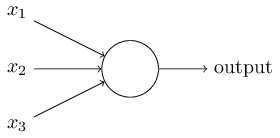
\includegraphics{perceptron}
	\centering
	\caption{Perceptron Model \protect \cite{nielsenneural}}
	\label{fig:1}
\end{figure}
\par
This model was improved and developed further in the 1960s by Frank Rosenblatt. He introduced weights (real numbers that express the importance of the input in relation to the output) \cite{rosenblatt_perceptron:_1958}. Because the neuron’s output can only be 0 (neuron isn’t activated) or 1 (neuron is activated), this can be determined through the sum of the weights being greater or less than a set threshold value (also a real number that is given as a parameter). This is called an activation function.
\begin{equation}
 output =
    \begin{cases}
      0 & if \quad \sum_{j}^{} w_j x_j \leq threshold\\
      1 & if \quad \sum_{j}^{} w_j x_j > threshold
    \end{cases}
\label{eq:1}
\end{equation}
\\
At a glance, one neuron on its own isn’t very impressive and it can only do so much through firing or not depending on the received input. One neuron by itself isn’t learning anything either, as the output will never vary if you give the same input over and over (threshold is still the same). There are two immediate ideas that surface into how to make a neuron useful and interesting: finding a way to make it learn, and grouping multiple neurons together that will form a (neural) network. \cite{marsland_machine_2015}
\subsection{Layered Neural Networks}
As previously noted, a single neuron can only do so much in order to make a decision, and a very simple one at that, but a complex network can make more complex decisions. Neural Networks are split between ‘layers’, the most simple one having 3 layers: an input layer, a hidden layer, and an output layer. All networks need to have 1 input layer and 1 output layer, but the hidden layer can be a group of layers, which is where all the computation is done.
\subsubsection{Shallow Neural Networks}
\begin{figure}[ht]
	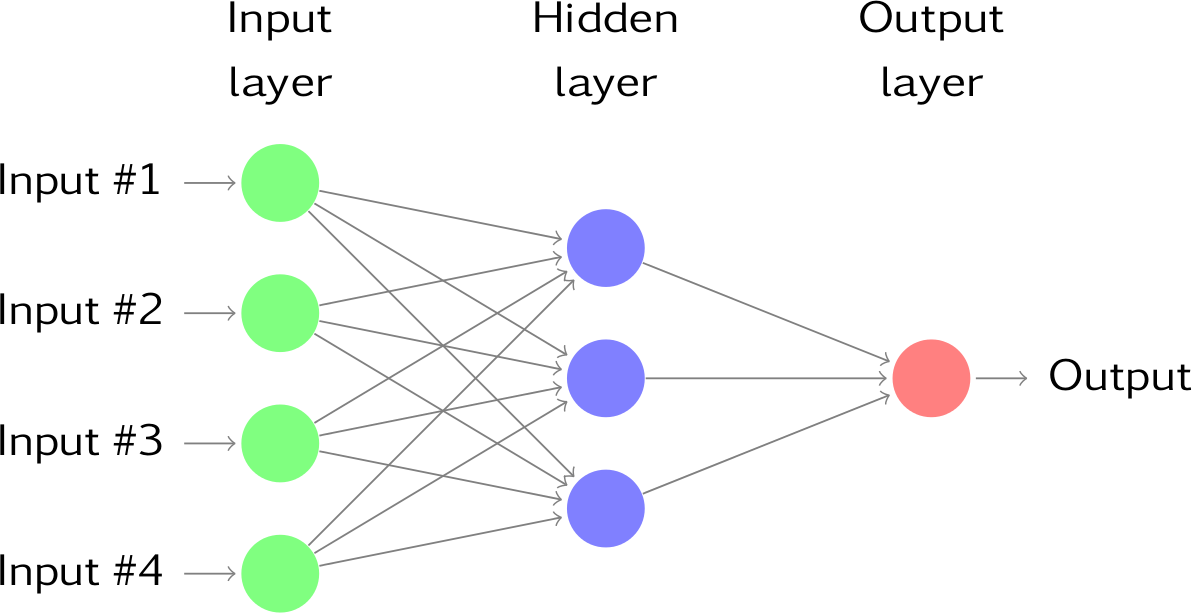
\includegraphics[width=\textwidth]{shallow}
	\centering
	\caption{Shallow Neural Network  \protect \cite{rob_j_hyndman_forecasting:_2018}}
	\label{fig:2}
\end{figure}
One might think of a neural network as a very complex system of layers, but in truth, the simplest neural network, also called a shallow NN, has an input and an output layer, as well as one (shown in [Figure \ref{fig:2}]) or sometimes two hidden layers.\par
As shown in the example NN, this neural network takes in 4 inputs and returns one output. The arrows that go from the input layer to the hidden layer shows that all the inputs are given to all the neurons of the network, and then all neurons return an output.
\subsubsection{Multi-Layer Neural Networks}
Multi-Layer NNs are more complex versions of the basic (shallow) model, by using more layers in the hidden layer. As all the computation is done by the hidden layer, multiple layers allow a neural network to do more abstract, complex computations.\par
Even though neural networks are not a new concept, they weren’t very popular in the 20th century, as there was not enough computing power to run them. As computers became better and better, also new methods for training neural networks were discovered. In 2006, the discovery of techniques for \textbf{deep} neural networks produced an important change that made deep neural networks and deep learning viable options that returned excellent results and performance in areas such as speech recognition, computer vision and natural language processing.  \cite{nielsenneural}

\subsection{Activation Functions}
After talking about the structure of a NN, the next step is learning about the decision-making aspect. Previously, we mentioned that a neuron activates or not depending on the calculation of the sum of the input weights. Determining this is the purpose of the activation function.\par
\subsubsection{Step Function}
The step function is the simple “if - then - else” version of activating a neuron, as seen in Equation \ref{eq:1}. As such, this can be the function to use for a binary application,  something that will return “yes/no” to a query. But then, if you want something more advanced and the output required has more than two options, the step function is no longer giving you a definite answer. For example, a NN that can tell you in which direction to go depending on the 4 cardinal points, if two of the neurons will fire North and West, it is unclear which one to pick: N? W? Or perhaps NW? For this scenario (which is a more real-life scenario anyway), the NN needs to give intermediate (analog) activation values rather than binary ones. \cite{sharma_understanding_2017}
\subsubsection{Linear Function}
A linear function (eg. f(x) = ax +b) is a function whose graph is a straight line. This way a NN will give a range of activations, where you can pick the biggest value (or values). But as a linear function is a constant function, if multiple layers in the same NN use linear functions, as the data moves through the functions, combining linear functions, is the equivalent of just a single linear function, meaning they can all be condensed into one single layer.
\subsubsection{Sigmoid Function}
A sigmoid function(e.g. f(x) =\( \frac{1}{1+e^x} \)) is a function who will produce a result between 0 and 1. The sigmoid function is one of the most used functions, and is most useful for training data between 0 and 1 (as bigger numbers of x will take the results to the extremes of the graph curve)[Figure \ref{fig:3}].
\begin{figure}[ht]
	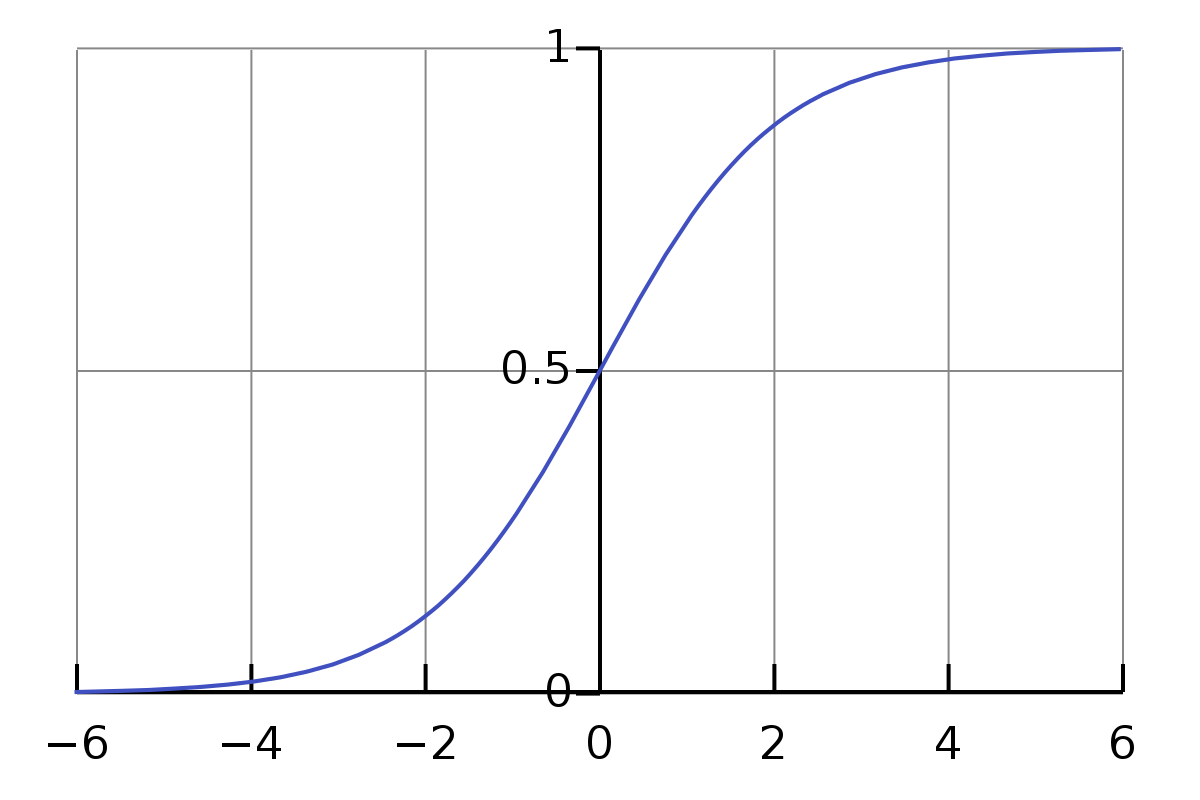
\includegraphics[width=\textwidth]{sigmoid}
	\centering
	\caption{Sigmoid Function Graph \protect \cite{nikhil_ketkar_deep_2017}}
	\label{fig:3}
\end{figure}

\subsection{Learning/Training Algorithms}
Having a model of a NN is only half of what a NN is and does. The big selling point of a NN is it’s learning capabilities, also referred to as machine learning, and its similarities to how humans learn. The definition given by Mitchell \cite{mitchell_explanation-based_1993} is that given a task, training experience, and a performance measure, a computer is said to learn if its performance of the task improves with experience.\cite{thrun_learning_2012}\par
These algorithms build a mathematical model based on sample data (also called training data) in order to generate decisions without any additional human programming. Machine learning can be split into three broad categories:
\begin{itemize}
	\item Supervised Learning, where an algorithm builds its model by having both the inputs and the desired results (used in speech recognition, handwriting recognition, etc.)
	\item Unsupervised Learning, where an algorithm builds its model by having only the inputs. Here, there is no correct answer from the start.
	\item Reinforcement Learning, where an algorithm is built around maximising its reward, based on rules given.
\end{itemize}
\subsubsection{Genetic Algorithms}
Genetic Algorithms are based on the real-life process of natural evolution \cite{agoston_e._eiben_introduction_2015}. Eiben notes that this approach is not surprising at all, as the power of evolution is present everywhere in the world, through its diversity and adaptability to any environment and specific issues. This inspiration is closely tied to the fundamental principle of trial-and-error, as it takes many generations to adapt a species to its full potential.\par
A genetic algorithm’s purpose is to optimise a set of parameters. This information is encoded in a bit string of fixed length, called the parameter string, or individual \cite{goldberg_genetic_1988}. Each individual is a different possible solution to the problem, the solution’s quality being measured through its fitness value (given by a fitness function specific to the problem). The evolution algorithm is a cycle of selection, crossover and mutation. By having an initial population, also called the first generation (usually randomly generated solutions), we want to select the best (fittest) individuals to be part of the parent pool for creating new offspring.\par
The crossover is the phase where offspring are created, this can be done through various means (list), this is the most significant phase of the algorithm as it dictates the future of the solutions.\par
Mutation is the step where some of an offspring’s genes are randomly modified, as to incentivise gene diversity. Mutation happens through a user defined mutation probability and can be done through a number of ways (inverting a bit in a binary gene, using uniform or non-uniform random values for integer or float genes, etc.).\par
Both the mutation probability and mutation size are usually set low, as using too much randomness defeats the purpose of the algorithm, turning it into a simple random function.\par
By doing this, evolutionary algorithms consider multiple points in the search space concurrently, reducing the risk of converging to local optima (Branke, 1995). Even though there is a significant degree of probability applied to every step, by favouring the fitter individuals, the most relevant areas of the search space are explored.\par
\subsubsection{Backpropagation}
Backpropagation (backward propagation of errors) is a widely used supervised learning algorithm, that through the use of an error function, the algorithm calculates the gradient of the function and determines if the NN has made a mistake when a prediction was made.\par
This algorithm is based on an evolutionary approach, as an untrained NN doesn’t know anything about what it needs to do, but through exposure (inputs) and a lot of trial and error (the training), the NN learns from the data provided, this being reflected in the weights (the way the NN alters the data through its layers), the more the NN is trained, those weights get calibrated and can make more accurate predictions.\par
Backpropagation works by propagating the input data \textbf{forward} through the NN layers, towards making a decision, and then \textbf{backpropagates} the error information of the prediction, in reverse through the layers, in order to adjust the weights.\cite{chris_nicholson_beginners_2019}  The steps the algorithm takes are:
\begin{itemize}
	\item NN makes a prediction about the data
	\item This is measured through a function
	\item The error is backpropagated to adjust the weights
\end{itemize}

\newpage
	\bibliographystyle{apacite}
	\bibliography{hons}
%example of References. See https://en.wikibooks.org/wiki/LaTeX/Bibliography_Management
%might be good to use a separate document for these so your main work is not one really long text file. 

%you can crate this on a extra tex document just like the title or any other part of the document.
\newpage
\begin{appendices}
\section{Project Overview}
%insert IPO

\begin{subappendices}
\subsection{Example sub appendices}
...
\end{subappendices}

\section{Second Formal Review Output}
Insert a copy of the project review form you were given at the end of the review by the second marker

\section{Diary Sheets (or other project management evidence)}
Insert diary sheets here together with any project management plan you have

\section{Appendix 4 and following}
insert content here and for each of the other appendices, the title may be just on a page by itself, the pages of the appendices are not numbered, unless an included document such as a user manual or design document is itself pager numbered.
\end{appendices}

\end{document}
